\chapter{Entwurf}\label{ref:chaptScript}
Der in diesem Kapitel beschriebene Entwurf zeigt konkret, wie das Konzept von
Masterly Mate umgesetzt werden wird. Hier werden Schemata und Architekturen
entwickelt, die im Kapitel \ref{ref:chaptImplementation} in Programmcode
umgesetzt werden.

\section{Realisierungsmethodik}
Nachdem in den vorangegangenen Kapiteln das Konzept von Masterly Mate erläutert
wurde, stellt sich die Frage nach einer geeigneten Möglichkeit zur Umsetzung. Da
die Anwendung stets verfügbar, leicht erreichbar, modular und einfach zu
verwalten sein soll, ist \ac{RoR} das Mittel der Wahl. Dieses bietet viele
interessante Features in Form von sogenannten gems, die dank einer regen
Community stets aktualisiert und erweitert werden. Zudem unterstützt es moderne
Programmierparadigmen, wie \ac{DRY} und \ac{KISS}. Dadurch bleibt die Anwendung
aus Sicht der Programmierer übersichtlich und erscheint sehr strukturiert. Das
das Framework der \ac{MVC}-Architektur folgt, schafft einen weiteren Grundstein
zur Trennung von Zuständigkeiten\footnote{bekannter unter "`separation of
concerns"'} und sorgt auch damit für Übersichtlichkeit. 

Weiterhin ist dieses Framework für die Weiterentwicklung im
OpenSource-Bereich prädistiniert, da damit bisher populäre
Webanwendungen, wie Twitter, realisiert wurden.

Darüber hinaus wird darauf geachtet, die Komponenten nach und nach nur dann zu
entwickeln, wenn sie tatsächlich gebraucht werden. Diese Vorgehensweise nach dem
\ac{YAGNI}-Prinzip beugt ein überlaufenes, unübersichtliches und schwer
zu wartendes Produkt vor.

\section{Internationalisierung}\label{ref:internationalisierung}
Die Internationalisierung gewährleistet eine Webanwendung, die möglichst
unabhängig von natürlichen Sprachen ist. Die Internationalisierung wird auch bei
Masterly Mate weitestgehend bereits in der ersten Version eingesetzt.

Die RoR API bietet dafür die Klasse I18n an, mit dessen Hilfe die
Internationalisierung durchgeführt werden kann. Die Bezeichnung I18n
kennzeichnet den Begriff Internationalisierung als Numeronym. Die Zahl 18 steht
für die Anzahl an Buchstaben, die zwischen den Buchstaben I und n liegen.
Die Klasse I18n bietet neben vielen anderen Methoden eine essentielle Methode
an, mit dessen Hilfe die Internationalisierung von Masterly Mate weitestgehend
realisiert werden kann. 

Die Methode trägt die Bezeichnung t als Kurzform für
translate. Diese Methode erwartet als einzigen Parameter eine Zeichenkette,
welche den Pfad zu dem entsprechenden Sprachstring angibt. Bei der
Initialisierung der RoR Anwendung Masterly Mate, werden sämtliche *.yaml Dateien
aus dem Verzeichnis \textit{config/locales/} als Sprachdateien geladen. Der Name
einer Sprachdatei sollte aus Konventionsgründen einer Rails Webanwendung, stets den
Ländercode beinhalten. In der ersten Version von Masterly Mate werden die
Sprachen Deutsch und Englisch unterstützt. 

Sven Fuchs bietet für sämtliche Sprachen auf
Github\footnote{\url{https://github.com/svenfuchs/rails-i18n/tree/master/rails/locale}} 
vorgefertigte Sprachdateien an. Diese Sprachdateien definieren für die jeweilige
Sprache entsprechende Formatierungen, wie z.B. Datum- und Zeitangaben. Aber auch
die Werte für Labels von Formularsteuerungskomponenten, wie z.B. die Submit-Schaltfläche, werden in
diesen Sprachdateien festgelegt. Die anwendungsspezifischen Strings müssen
selbstverständlich selbst in *.yaml Sprachdateien definiert und im Verzeichnis
\textit{config/locales/} abgelegt werden. 

Eine RoR Sprachdatei ist hierarchisch aufgebaut. Die einzelnen Hierarchieebenen
werden dann später beim Zugriff auf ein Sprachstring über ein Punkt voneinander
getrennt. Grundlegend definiert man eine von der natürlichen Sprache unabhängige
Zeichenkette dadurch, indem ein fester Bezeichner gefolgt von einem Doppelpunkt
definiert wird. Nach dem Doppelpunkt folgt die sprachabhängige Zeichenkette. Im
Programmcode wird an den Stellen, an denen eine sprachenunabhängige Zeichenkette
ausgegeben werden soll, die Methode t der Klasse I18n eingesetzt und dieser als
Parameter der Pfad zu dem entsprechenden Bezeichner übergeben.

Masterly Mate ist bis auf die vom Nutzer erstellten WBTs vollständig für die
Sprachen Deutsch und Englisch Internationalisiert. Einige WBT-Engines bieten
den Mechanismus zur Internationalisierung nicht an. Aus diesem Grund wurde
dieses Vorhaben im Rahmen dieser Studienarbeit vernachlässigt.

\section{Beschreibung des Entwurfsklassendiagramms und
Use-Case}\label{ref:classModel}

\subsection{Use-Case Diagramm}
Im Use-Case Diagramm aus Abbildung \ref{ref:picUseCaseDia}, sind die einzelnen
benötigten Komponenten enthalten, wie sie die Analyse ergeben hat. Zunächst
lassen sich Aktoren ausmachen, welche in System/Software-Aktoren und menschliche
Aktoren aufteilen lassen.

\begin{figure}[ht]
\centering
\includegraphics[width=1\textwidth]{UseCaseDia.png}
\caption{Use-Case-Diagramm von Masterly Mate}\label{ref:picUseCaseDia}
\end{figure}

Bei den Softwareseitigen Aktoren ergab die Analyse als Aktoren den Webserver,
ein Einzelnes WBT (sie sollen nach Abschluss die Punkte im System eintragen),
das Autorenwerkzeug und den Webbrowser. Auf der Seite der Aktoren ließe sich der
Lernende (Standard-User), Tutor, Autor und Admin ermitteln. Zu beachten ist,
dass die Aufteilung der menschlichen Aktoren auch eine Berechtigungshierarchie
darstellt, wobei ein Lernender die geringsten und ein Admin die meisten
Berechtigungen hat.

Die einzelnen Use Cases werden nun jeweils im folgenden kurz beschrieben. Zu
beachten ist dabei zusätzlich, dass diese Analyse sich nicht zwingend mit dem
Ergebnis aus der Studienarbeit deckt, da Funktionalitäten auf spätere Releases
verschoben worden sind.

\subsubsection{WBT durcharbeiten} 
Agierende Aktoren: \begin{itemize}
  \item WBT
  \item Lernender
  \item Tutor
  \item Autor
  \item Admin 
\end{itemize}

Ein Benutzer startet ein WBT und schließt es erfolgreich ab bzw.
scheitert oder beendet es vorzeitig. Im Anschluss daran, werden die erreichten
Punkte im System eingetragen. In der Version der Studienarbeit, wird dies noch
vom Benutzer selbst durchgeführt. Später soll dies das WBT übernehmen.
\newpage
\subsubsection{Bewerten}
Agierende Aktoren: \begin{itemize}
  \item Lernender
  \item Tutor
\end{itemize} 

Den Use Case Bewerten gibt es in zwei Ausprägungen. Die erste Ausprägung ist die
Bewertung eines Tutors. Hat ein Lernender oder eine anderer Tutor (im folgenden
beide als "Lernende" bezeichnet) von dem Betreffenden Benutzer Hilfe erhalten,
so kann der Lernende im Anschluss daran diese Hilfe im System bewerten.
Dies kann er mit Sternen und wahlweise mit einem Kommentar tun (Kommentar noch
nicht in der Alpha-Version). Die Zweite Ausprägung ist die Bewertung eines WBTs.
Ein Benutzer muss das WBT dafür abgeschlossen haben. Ebenso wie beim Tutor kann
er dies über Sterne und Kommentare tun.
	
\subsubsection{Sprachen verwalten}
Agierende Aktoren: \begin{itemize}
  \item Alle menschlichen Aktoren (Ausprägung Sprache
hinzufügen kann nur der Admin)
\end{itemize}

Ebenso wie im obigen Use Case gibt es hiervon zwei Ausprägungen.
Nummer Eins ist der Use Case Sprache wechseln. Dieser kann von jedem Benutzer
durchgeführt werden und bewirkt, dass alle Zeichenketten in MasterlyMate, welche
in der betreffenden Sprache vorhanden sind, ausgetauscht werden. Use Case Nummer
Zwei kann nur von einem Administrator durchgeführt werden. Und bewirkt die
Erzeugung einer weiteren Sprache, welche eingestellt werden kann. Gegenwärtig
wird dies noch direkt durch eine Änderung der Sprachdateiten getan.
\newpage
\subsubsection{Profil verwalten}
Agierende Aktoren: \begin{itemize}
  \item Alle menschlichen Aktoren
\end{itemize}

Auch dieser Use Case verfügt über zwei Ausprägungen. Der erste Use Case ist das
bearbeiten eines Profils. Dies kann nur der besitzer des jeweiligen Profils.
Den anderen Use Case kann hingegen jeder Benutzer durchführen. Es handelt sich
dabei um das Betrachten eines Profils. Dies ist insbesondere für die
Kontaktaufnahme eines Benutzers zu einem Tutor notwendig.

\subsubsection{Suchen}
Agierende Aktoren: \begin{itemize}
  \item Alle menschlichen Aktoren
\end{itemize}

Es können sowohl Tutoren als auch WBTs gesucht werden. Dabei wird jeweils
berücksichtigt welches Themengebiet gefragt ist.
	
\subsubsection{Themengebiet abfragen}
Agierende Aktoren: \begin{itemize}
  \item Webserver
\end{itemize}

Der Webserver überprüft bei einer Suchanfrage die einzelnen Themen.
	
\subsubsection{Themen verwalten}
Agierende Aktoren: \begin{itemize}
  \item Admin
  \item Webserver
\end{itemize}

Nur der Admin kann die beiden Ausprägungen dieses Use Cases durchführen, welche
das Hinzufügen und Löschen eines Themas darstellen.
	
\subsubsection{WBT verwalten}
Agierende Aktoren: \begin{itemize}
  \item Admin
  \item Autor
  \item Webserver
\end{itemize}

Dieser Use Case besitzt drei Ausprägungen. Admin und Autor können WBTs
einbinden. Es kann jedoch nur der User, welcher ein WBT eingebunden hat, dieses
auch wieder entfernen bzw. ersetzen. Dies gilt nicht, wenn der betreffende
Benutzer ein Administrator ist. Dieser kann jedes WBT löschen oder ersetzen.
	

\subsection{Entwurfsklassendiagramm}
In dem Entwurfsklassendiagramm aus Abbildung \ref{ref:picKlassendia}, sind die
Modelle und ihre Beziehungen zueinander dargestellt. Diese Modelle bilden
einzelne Konzepte im System ab. 

So stellt User ein Zentrales Modell dar, welches als Abbildung eines Benutzers
im System für die Authentifizierung verantwortlich ist. Außerdem werden dem User
verschiedene Themen und WBTs zugeordnet. Diese Verbindungen benötigen jeweils
Assoziationsklassen. Dies liegt daran, dass es in dieser Verbindung Attribute
gibt, welche sich nicht eindeutig User oder WBT bzw. Thema zuordnen lassen.

Bei der Verbindung User-Thema benötigt man ein Attribut für die Punkte, welche
bisher von dem User in dem System erziehlt worden sind. Außerdem muss klar sein
welchen Rang ein User in dem jeweiligen Thema inne hat.

Die Verbindung User-WBT dagegen benötigt eine Variable um zu hinterlegen ob ein
User das WBT bereits einmal abgeschlossen hat und wenn ja, wie viele Punkte er
erreicht hat. 

Im folgenden wird auf die Modelle des UML-Diagrammes näher
eingegangen. Dazu sei angemerkt, dass zwischen einem realen Konzept und dem
des Models underschieden wird. D.h. wenn z.B. im Folgenden vom User die Rede
ist, dann ist hierbei das Model oder eine Instanz der User-Klasse gemeint. Wird
hingegen vom Benutzer gesprochen, so ist auch tatsächlich jener gemeint.

\begin{figure}[ht]
\centering
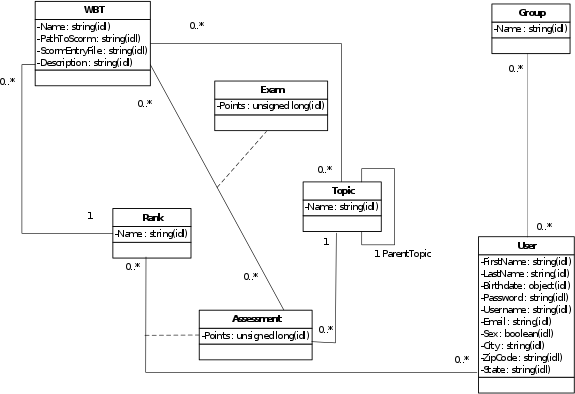
\includegraphics[width=1\textwidth]{Klassendiagramm.png}
\caption{Entwurfsklassendiagramm von Masterly Mate}\label{ref:picKlassendia}
\end{figure}

\subsubsection{WBT}\label{ref:objectWBT}
Das WBT-Model verfügt über eine ID, sowie über einen Pfad zur eigentliche
SCORM-Datei. Wie bereits erwähnt ist es einem oder mehreren Themen (Topics)
zugeordnet. Auf Datenbankseite bedeutet dies, dass eine Zwischenentität zwischen
Topic und WBT eingeführt werden muss. 

\subsubsection{Topic}
Im UML-Diagramm ist ersichtlich, dass das Model Topic eine referenz auf sich
selbst besitzt. In dieser Referenz kann ein Topic sowohl die Rolle des über- als
auch des Unterthemas bekleiden. Unterthemen dienen einer genaueren Unterteilung
der WBTs. Tobics werden mit ihrem Namen identifiziert. Dies gilt auch für die
übergeordneten Topics. Dies bedeutet, dass ein Unterthema die Information
besitzt, zu welchem Topic es gehört. Diese vorgehensweise ist auch für die
Datenbank hilfreich, da so der Maxime entsprochen wird, den Fremdschlüssel auf
der N-Seite zu notieren.

\subsubsection{User}
Das Dritte große und wahrscheinlich sogar größte Model ist der User. Er ist
gekennzeichnet durch einen Benutzernamen, Vor- und Nachname, Passwort,
Geburtstag und einer Email-Adresse. Der User, stellt die Benutzer im System dar.
Er wird für die Registrierung und Authentifizierung verwendet. Des Weiteren
werden ihm die Punkte zugeordnet, welche ein Registrierter Benutzer in einem WBT
erzielt. Damit werden ebenso die Ränge dem Benutzer zugeordnet, von welchen er
beliebig viele haben kann (siehe dazu Model: Ränge). 
Ein Benutzer ist außerdem in einer oder mehrerer der möglichen Gruppen
eingeordnet.
Über diese wird geregelt, welche berechtigungen er im System hat. Näheres dazu
ist im entsprechenden Abschnitt zu finden.
Eine besondere Funktion fällt der Zuordnung eines User zu einer Location zu. Mit
ihr ist es möglich, dass Benutzer Tutoren in der Nähe ihrer eigenen Wohnstätte
finden können (Auch dazu, sie im entsprechenden Abschnitt).

\subsubsection{Group}
Die Gruppen werden zur Festlegung der Berechtigungen verwendet. Ein User
kann in beliebig vielen Gruppen sein und diese wiederum kann beliebig viele User
enthalten. Die Gruppen im System sind die Administratoren, welche volle Rechte
im System besitzen. Die etwas schwächeren Tutoren können WBT hochladen und ihr
eigenes löschen. Außerdem können sie von anderen Usern bewertet werden. Die
Dritte vorhandene Gruppe sind die normalen User. Diese können lediglich WBTs
durcharbeiten, Profile von anderen Usern einsehen, sowie ihr eigenes bearbeiten.
Implizit vorhanden, jedoch nicht implementiert sein soll die Gäste-Gruppe. Diese
umfasst alle Benutzer, welche keinen User im System besitzen.

\subsubsection{Location}
Eine Location beschreibt den groben Standort an dem ein Benutzer wohnt. Daher
verfügt dieses Model auch nicht über die kompletten Adressdaten eines Benutzers,
sondern nur über die Stadt, die Postleitzahl sowie das Land. Da die Location
einzig den Sinn hat, die Suche nach geeigneten Tutoren einzugrenzen ist eine
genauere Standortsbestimmung nicht notwendig. Da es mehrere User gegen kann, die
der gleich Location zugeordnet sind, ist wird diese auf der User-Seite durch die
entsprechende ID der Location identifiziert. 

\subsubsection{Assessment}
Das Assesment bildet als Assoziationsklasse zwischen User und Topic die
Beziehung zwischen dem User und einem Topic ab. In ihr wird gespeichert, wie
viele Punkte er durch die Absolvierung von WBTs in einem Thema erreicht hat.
Entsprechend zeigt das Assesment auch den Rang an, den ein Benutzer in einem
bestimmten Thema erreicht hat.

\subsubsection{Rank}
Der Rang eines Benutzer spiegelt den Erfahrungsstand wieder, den ein Benutzer in
einem Thema erreicht hat. Er wird bei entsprechender Punktzahl (Erspielte Punkte
bzw. Sterne) vom System vergeben.

\section{Funktionalitäten aus Nutzersicht}
Prinzipiell ist Masterly Mate aus zwei Komplexen aufgebaut. Zum einen kann sich
ein Nutzer fachlich weiterbilden. Zum Anderen bietet ein Nutzer als Tutor seine
Hilfe für ein bestimmtes Fachgebiet an.

\subsection{Masterly Mate für Lernende}
Aus Sicht der Lernenden baut sich Masterly Mate aus den folgenden Komponenten
auf.

\subsubsection{Registrieren und Einloggen}
Ein neuer Nutzer wird sich zunächst registrieren. Ist dies bereits geschehen,
kann er sich einloggen und sich dem Bearbeiten von WBTs oder der Administration
seines Profils widmen.

\subsubsection{Durcharbeiten von WBTs}
Ist ein Nutzer an Weiterbildungsangeboten interessiert, so geht er ein oder
mehrere WBTs durch. Dazu erhält er nach einer passenden Filterung der Ergebnisse
anhand einer Themenwahl und des dazugehörigen fachlichen Ranges (siehe Abschnitt
\ref{ref:autoResult}) eine verfügbare Liste an WBTs, die er nach seinem Gusto
bearbeiten kann.

\subsubsection{Tutorensuche}
Stößt der Lernende beim Durcharbeiten von WBTs auf ein fachliches Problem, so
kann er einen Tutor aufsuchen. Die Darbietung passender Tutoren erfolgt ebenso
nach einer automatischen Filterung. Die Filterung wird auch hier anhand des
fachlichen Rangs des Lernenden und des Themengebiets vorgenommen. Hinzu kommt
der didaktische Rang des Tutoren und die jeweils angegebene Postleitzahl
Lernenden und des Tutors, sodass ein Treffen aufgrund der räumlichen Nähe
einfacher möglicht wird.

\subsubsection{Profil administrieren}
Jedem Nutzer ist es erlaubt, sein eigenes Profil zu administrieren. Dort kann er
sein Profilbild und andere persönliche Angaben, wie Spitzname, Name und
Postleitzahl ändern. Zusätzlich kann er hier eine Option anhaken, die ihm zum
Tutor macht. Damit erscheint er für andere Lernende in den Suchergebnissen für
passende Tutoren. Demgegenüber kann er den Haken wieder entfernen, falls er kein
Tutor mehr sein möchte.

\subsubsection{Navigation, Impressum, Kontakt}
Eine übersichtliche und nicht zu detailierte Navigation für Masterly Mate war
ebenfalls ein Ziel dieser Studienarbeit. Die Funktionsweise eines
Navigationsmoduls sollte nicht neu entwickelt werden. Aus diesem Grund wurden
einige vorgefertigte Gems für die Navigation in Betracht gezogen. 

Das Gem, welches letztlich für die Navigation in Masterly Mate eingesetzt wurde,
nennt sich Simple-Navigation\footnote{\url{https://github.com/andi/simple-navigation}}.
Die Handhabung dieses Gems ist sehr einfach und darüber hinaus bietet es eine
übersichtliche Infrastruktur und somit ein Grundkonzept für die Funktionsweise
einer Navigation. Die Elemente der Navigationsleiste werden an einer zentralen
Stelle in der config/navigation.rb definiert. Auch das Festlegen von
Subelementen ist möglich. Weiterhin kann man eine von mehreren 
Darstellungsarten, wie z.B. einer ungeordneten HTML Liste, Linklisten,
Breadcrumbs, etc. für das Navigationsmoduls auswählen. 

Für Masterly Mate wird eine entsprechend mit CSS formatierte Linkliste
eingesetzt. Für das Impressum wurde im Rahmen dieser Studienarbeit keine eigene
Seite in der Webanwendung vorgesehen. Dieses befindet sich daher in der Fußleiste von
Masterly Mate. Auch ein Kontaktformular wurde in dieser Arbeit nicht vorgesehen.
Der Kontakt erfolgt in der aktuellen Version über das Anschreiben an die
Entwickler von Masterly Mate per E-Mail. 

\subsubsection{Themen}
Themen fungieren für den Benutzer zum Einen als Suchfilter bei der Suche nach
den WBTs. Dies sorgt dafür, dass der Benutzer ohne umschweife auf WBTs zugreifen
kann, welche für ihn interessant sind. Außerdem dienen Themen dazu, die
unterschiedlichen Ränge, welche ein Benutzer zur selben Zeit in Masterly Mate
haben kann, voneinanderabzugrenzen. Jeder Benutzer kann in einem Thema nur genau
einen Rang inne haben. Umgekehrt kann er jedoch in beliebig vielen Themen einen
Rang haben.

Zu diskutieren ist, hierbei ob ein Benutzer jeweils in einzelnen Unterthemen
einen Rang inne hat und auch im Oberthema oder nicht. Wenn er in jedem wirklich
Thema einen Rang inne haben kann ist außerdem zu klären, wie sich das auf den
Rang im Überthema auswirkt. Er könnte in diesem Falle sowohl die erzielten
Punkte gutgeschrieben bekommen als auch in allen darüberliegenden Themen. Dann
hätte er in dem Überthema einen Rang, welcher mindestens so hoch ist, wie der
höchste Rang in einem der Unterthemen.
 
In einem anderen Falle, namentlich Ränge in allen Themen ohne das kaskadieren
der Punkte, wäre es möglich, dass der Benutzer in einem Unterthema Meister sein
könnte im Übergeordneten jedoch nur Erfahrener, da er in dem Überthema nur die
Punkte erhält, welche direkt diesem Thema untergeordnet sind.

Ein ganz anderer Fall hingegen wäre es, wenn der Benutzer nur in einem der
Überthemen einen Rang haben könnte und die Unterthemen einzig und allein der
Unterteilung dienen. In diesem Falle müsste man im Datensatz nachprüfen ob das
Thema, zu dem das abgeschlossene WBT gehört, ein übergeordnetes Thema hat. Ist
dies der Fall so müssten dieses Thema überprüft werden. Dieser Vorgang müsste
solange fortgesetzt werden, bis das hierarchisch höchste Thema gefunden ist.
In diesem Thema würden dann die Punkte dem Benutzer zugeteilt.

Ein ganz anderes Problem stellt das löschen von Themen dar. Auch hier gibt es
mehrere Möglichkeiten. So ist es denkbar, dass bei einer Löschung eines Themas,
alle Unterthemen mit WBTs gelöscht werden. Dies sollte allerdings mit Vorsicht
genossen werden und am besten mit einer oder eventuell zwei Abfragen hinterfragt
und bestätigt werden.

Eine andere, weniger gefährliche Option wäre es, die enthaltenen Unterthemen und
WBTs dem übergeordneten Thema des gelöschten Themas zuzuordnen. In diesem Fall
ist es notwendig ein Root-Thema zu definieren, welches alle Themen beinhaltet.
In diesem Falle könnte es allerdings Themen geben, die nur in dem Root-Thema
enthalten sind. D.h. es müsste möglich sein in diesem Thema einen Rang
zu erhalten (Man könnte sich an dieser Stelle fragen ob es nicht Sinvoll wäre,
dort ein WBT zur "`frage nach dem Leben, dem Universum und Allem"' zu
platzieren, weiter sei die Frage erlaubt, ob ein Meister in diesem Thema sich
``Master of the Universe'' zu nennen habe). Alternativ könnte man abfragen ob
ein WBT sich nur innerhalb des Root-Themas befindet und wenn dies der Fall ist,
dem Benutzer den Zugriff verwehren.  

\subsection{Masterly Mate aus Sicht eines Tutors}
Ein Tutor ist quasi eine erweiterte Form eines Lernenden. So bleiben dem Tutor
die verfügbaren Möglichkeiten eines Lernenden erhalten. Hinzu kommen zwei
weitere Funktionen.

\subsubsection{Lernende unterstützen}
Lernende werden gelegentlich an ihre Grenzen stoßen und Tutoren zu Rate ziehen.
Als Tutor auf Masterly Mate ist man, da man sich selbst in beliebigen
Fachgebieten weiterbilden kann, mit einem Lernenden nahezu gleichgestellt. Dem
Lernenden wir damit eine Hilfe gebende Person auf Augenhöhe vermittelt. 

Im Konzept von Masterly Mate ist nur eine Hilfe der beschriebenen Art
berücksichtigt. Tutoren können sich jedoch darüber hinaus auch auf eine
beliebige andere Art an Lernende wenden, wie zum Beispiel das geben von
Workshops oder halten von Präsentationen.

\subsubsection{WBTs verbessern und hinzufügen}
Hat ein Tutor den Rang des Meisters erreicht, so ist es ihm aufgrund seiner
herausragenden didaktischen Leistungen erlaubt, bestehende WBTs zu verbessern
oder neue zu entwickeln und auf die Plattform zu laden.